\chapter{SetUID}

\section{Comandi Linux}

\begin{itemize}
    \item \textbf{Aggiungere Utenti}: from /etc/password file or \textit{add user}. 
    Ogni Utente ha un Unique ID e può appartenere a uno o più gruppi $ \rightarrow $ definisce autorizzazioni.
    \item \textbf{Cambiare Utente}: \textit{su user\_name}
    \item \textbf{Creare Gruppo}: \textit{sudo groupadd group\_name}
    \item \textbf{Aggiungere Utente a Gruppo}: \\\textit{sudo usermode -a -G group\_name user\_name}
    \item \textbf{Composizione Gruppi}: from /etc/group (/etc/sudoers) file or \textit{groups} or \textit{id}
\end{itemize}


\section{Tipi di Accessi a File e Directory}

\begin{itemize}
    \item \textbf{R: READ - 4}
    \item \textbf{W: WRITE - 2}
    \item \textbf{X: EXECUTE - 1}
\end{itemize}

\begin{figure}
    \centering
    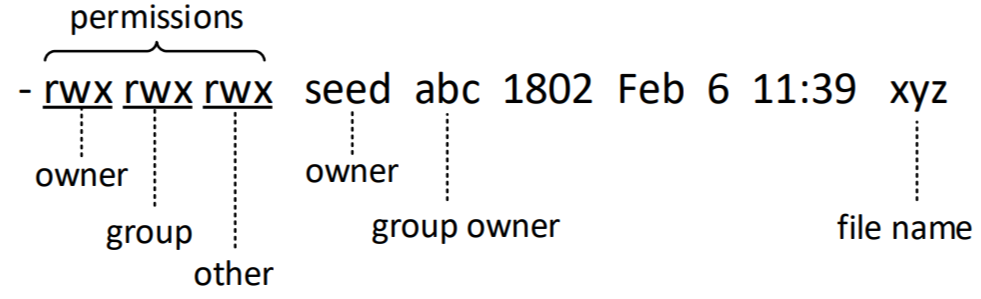
\includegraphics[width=0.75\linewidth]{chapters/images3/autorizzazioni-file.png}
\end{figure}


\section{Programmi Privilegiati: Set-UID}

\begin{itemize}
    \item \textbf{Demoni}
    \begin{itemize}
        \item processo eseguito in background, solo come root o altri utenti privilegiati.
    \end{itemize}
    \item \textbf{Programmi Set-UID}
    \begin{itemize}
        \item Ampiamente utilizzati nei sistemi UNIX, programma contrassegnato con un bit speciale.
    \end{itemize}
\end{itemize}


\section{Attacchi Basati su Set-UID}

\textbf{Meccanismo Set-UID:} l'utente esegue un processo con i privilegi del proprietario del programma. 

\subsection{Privilege Escalation to execute programs:}
\begin{itemize}
    \item \texttt{cp /bin/cat ./mycat}: crea il programma \texttt{mycat} come copia di \texttt{cat}.
    \item \texttt{sudo chown root mycat}: cambia il proprietario di \texttt{mycat} a \texttt{root}.
    \item \texttt{mycat /etc/shadow}: non eseguito poiché \texttt{mycat} non ha i privilegi Set-UID.
    \item \texttt{sudo chmod 4755 mycat}: abilita bit Set-UID per \texttt{mycat} (4 $\rightarrow$ \textit{EUID = RUID Process Owner}).
    \item \texttt{mycat /etc/shadow}: ora eseguito con privilegi elevati, consentendo l'accesso a \texttt{/etc/shadow}.
\end{itemize}

\noindent Se il programma è di proprietà di \texttt{root}, viene eseguito con i privilegi massimi (EUID = 0). Il controllo degli accessi si basa sull'EUID $\rightarrow$ identifica i privilegi del processo eseguito.

\subsection{Privilege escalation to root shell:}
\begin{itemize}
    \item \texttt{gcc -o catall catall.c}: compila il file sorgente e genera un eseguibile chiamato \texttt{catall}.
    \item \texttt{sudo chown root catall}: cambia il proprietario di \texttt{catall} a \texttt{root}.
    \item \texttt{catall /etc/shadow}: non eseguito poiché \texttt{catall} non ha i privilegi Set-UID.
    \item \texttt{sudo chmod 4755 catall}: abilita bit Set-UID per \texttt{catall} (4 $\rightarrow$ \textit{EUID = RUID Process Owner}).
    \item \texttt{catall /etc/shadow}: ora eseguito con privilegi elevati, consentendo l'accesso a \texttt{/etc/shadow}.
    \item \texttt{catall "random; /bin/sh"}: esegue il programma \texttt{catall} passando come secondo arg \textit{/bin/sh} per ottenere una shell di root se il programma è eseguito con privilegi Set-UID.
\end{itemize}

\noindent \textbf{Nota:} In Ubuntu 16.04, \texttt{/bin/sh} punta a \texttt{/bin/dash}, che ha una contromisura: 
\begin{itemize}
    \item il programma perde i privilegi quando viene eseguito all'interno di un processo Set-UID. 
\end{itemize}
Pertanto, nell'attacco descritto, otterremo solo una shell normale. Per rimuovere questa contromisura, è possibile eseguire le seguenti operazioni:
\begin{itemize}
    \item \texttt{sudo -ln -sf /bin/zsh /bin/sh}: prima dell'exploit, creazione link simbolico di \texttt{sh} a \texttt{zsh}:
    \begin{itemize}
        \item \textbf{zsh non ha la stessa contromisura}
    \end{itemize}
    \item \texttt{sudo -ln -sf /bin/dash /bin/sh}: dopo l'exploit, ripristino link simbolico originale.
\end{itemize}

\section{Variabili d'ambiente}

Un insieme di valori dinamici. Fanno parte dell'ambiente operativo in cui viene eseguito un processo.

Un possibile esempio è la variabile \textit{PATH}.


